\section{Results}

\subsection{Robust Predictive Performance Across Hydrological Stations}

Before interpreting the internal knowledge structures of the model, it is essential to verify that the model achieves reliable predictive performance across hydrological stations\cite{ReviewOfXAI}. In this study, predictive performance is evaluated using the NSE, with a threshold of NSE $>$ 0.5 indicating satisfactory model performance\cite{Nse}.

\begin{figure}[ht]
    \centering
    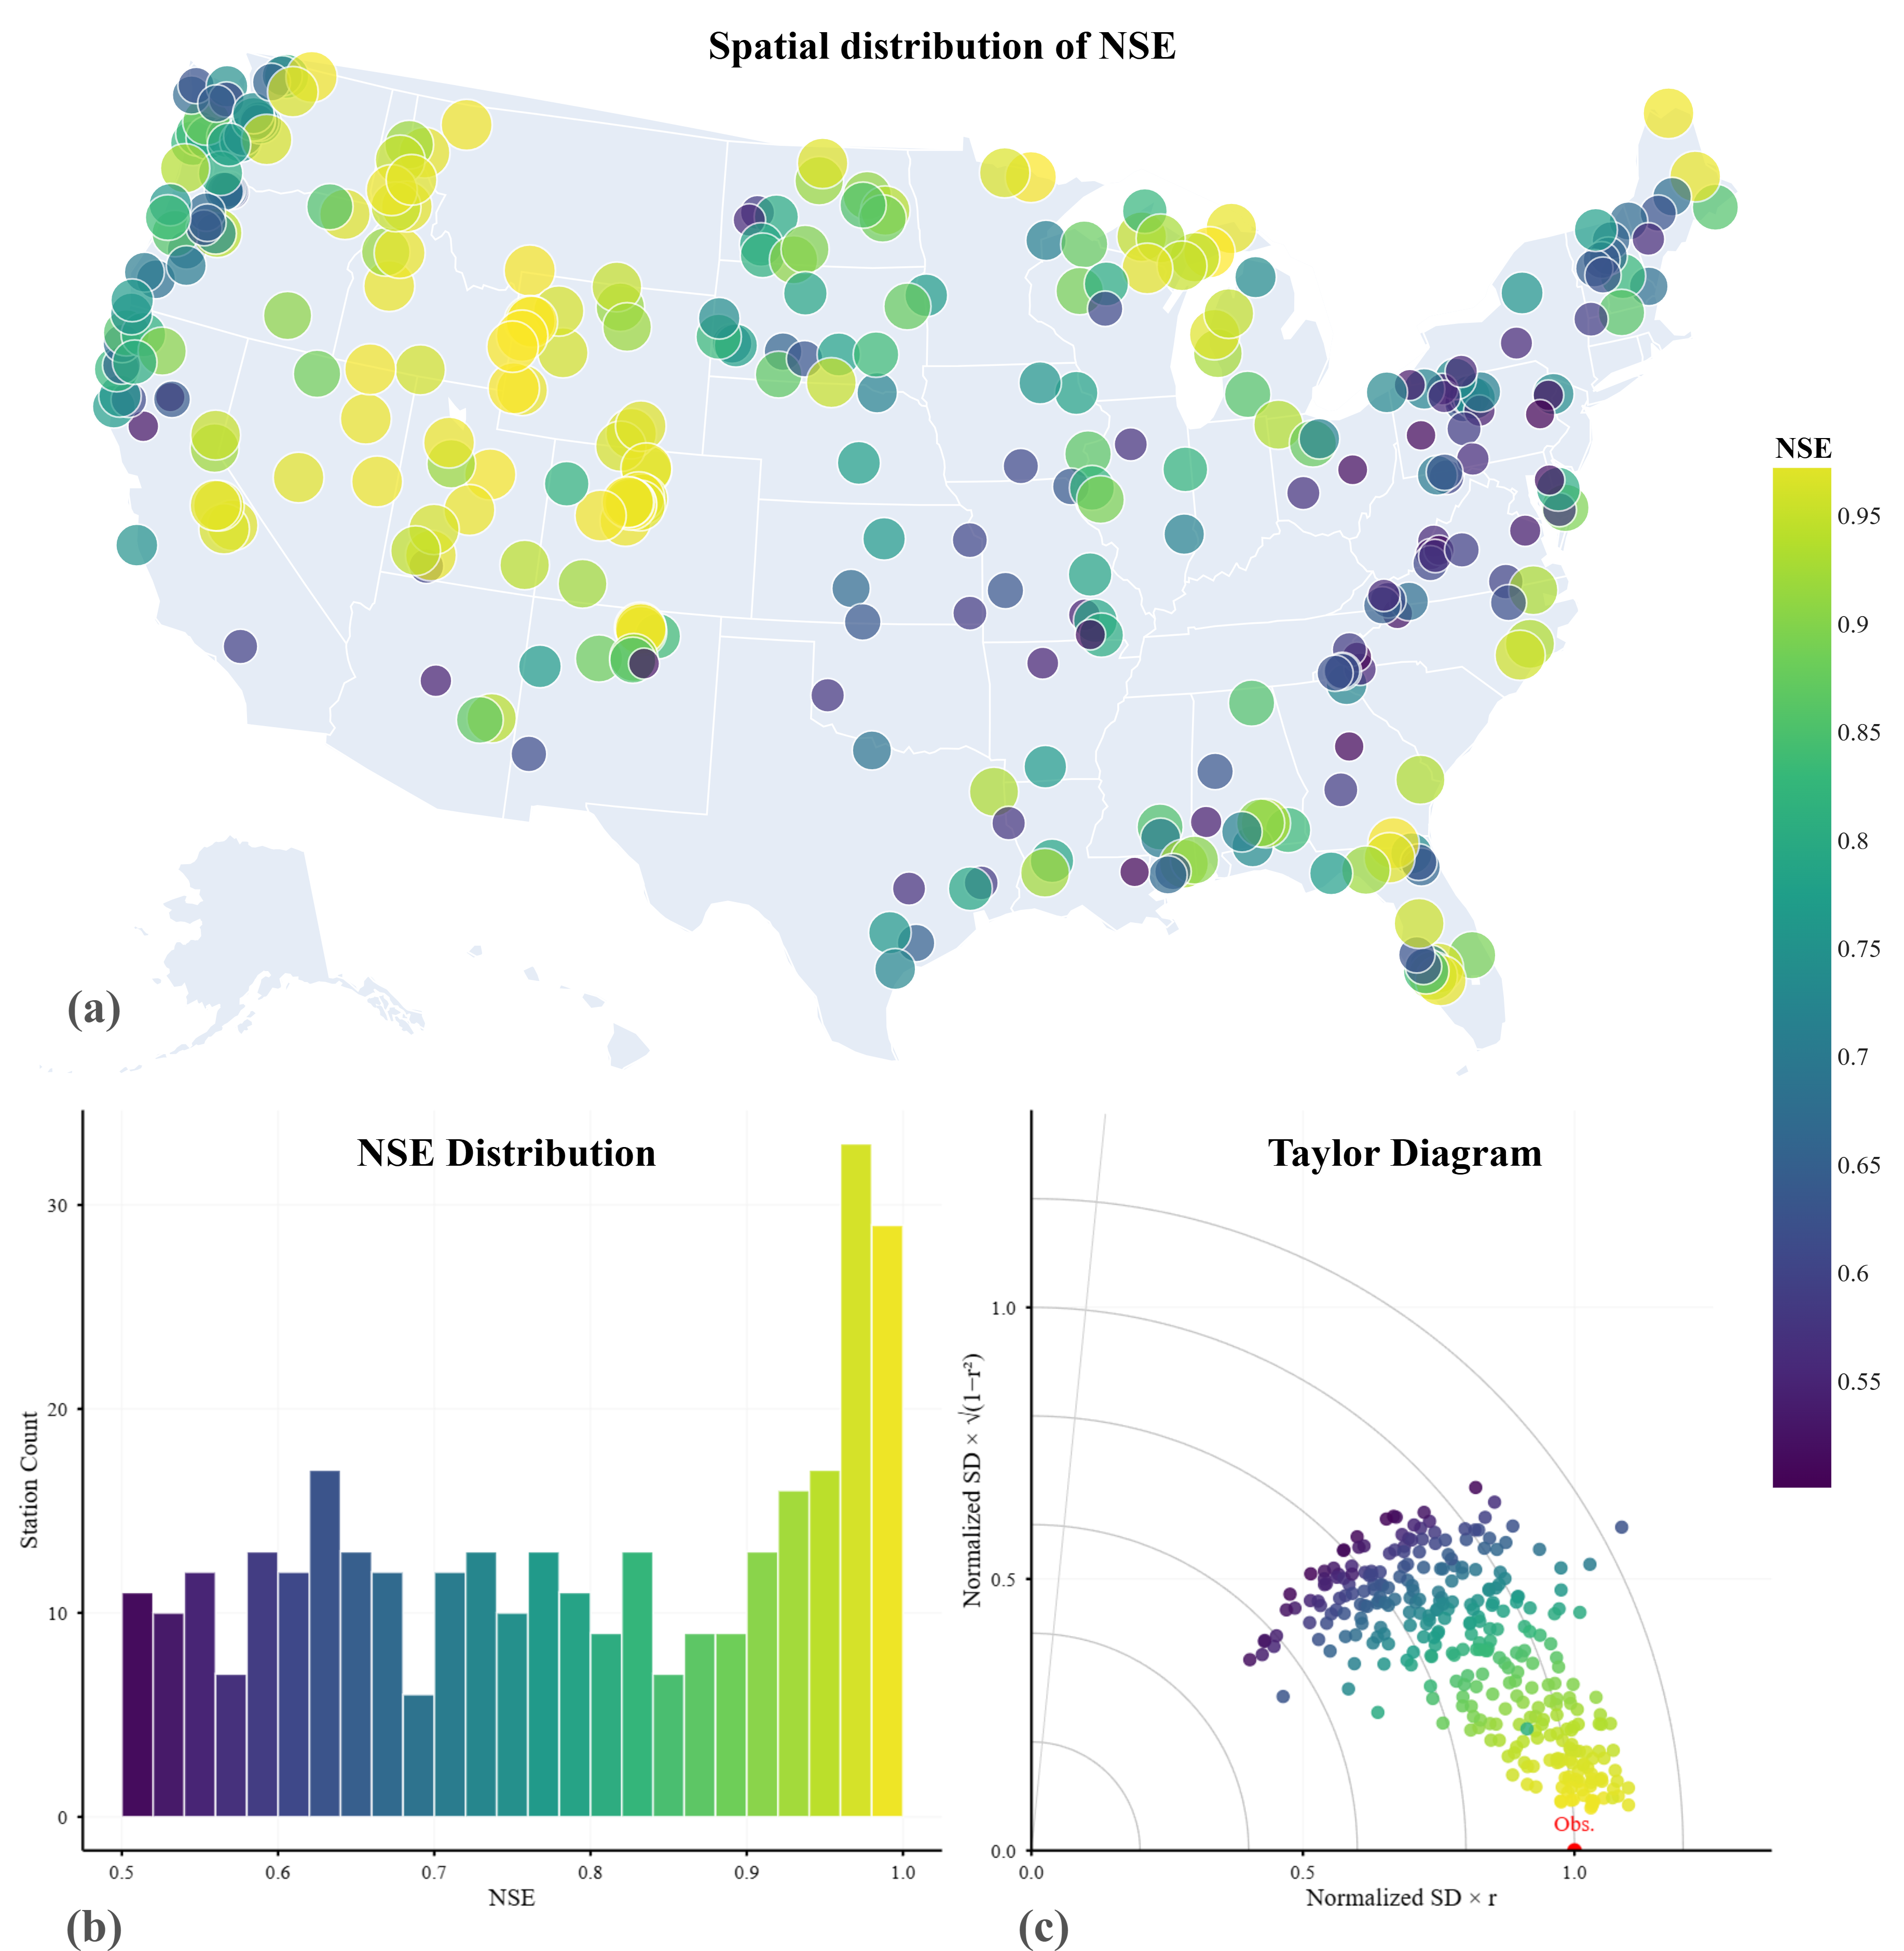
\includegraphics[width=\textwidth]{Figures/Fig3 Model Prediction.png}
    \caption{\textbf{Model performance across 521 streamflow gauging stations.} (a) Spatial distribution of NSE, with warmer colors indicating higher predictive skill. (b) Distribution of NSE values across all stations, showing that the majority achieve satisfactory performance (NSE $>$ 0.5). (c) Taylor diagram summarizing model performance in terms of correlation, normalized standard deviation, and centered root-mean-square error relative to observations. Overall, the results demonstrate that the model provides robust predictions for a large proportion of stations, while performance varies across regions, reflecting differences in hydrological conditions.}
    \label{nseDistribution}
\end{figure}
\FloatBarrier

As shown in Fig.~\ref{nseDistribution}, the STEH framework demonstrates robust performance across a large proportion of stations, despite being specifically designed to enhance interpretability rather than maximize predictive accuracy. Specifically, 327 out of 521 stations (approximately 62.8\%) achieve NSE values greater than 0.5, indicating satisfactory predictive skill in the majority of cases\cite{WRR_RMSE}.

This result suggests that the model is capable of capturing the dominant hydrological dynamics in most basins\cite{WRR_NSE}, thereby providing a reliable foundation for subsequent interpretability analysis\cite{ReviewOfXAI}. Consequently, the insights derived from the STEH framework are grounded in meaningful predictive behavior rather than artifacts of poor model performance\cite{hess-camels}.Based on this reliable predictive foundation, we next investigate the internal circuit structures of the model.



\subsection{Interpretable Circuit Structures Across Hydrological Stations}
Given the large number of stations (521), it is impractical to visualize the learned circuits for all stations individually. Therefore, a representative sampling strategy is adopted to systematically examine circuit structures under different predictive conditions.

Specifically, stations are categorized into three performance groups\cite{Nse} based on the NSE. One representative station is selected from each category, as summarized in Table~\ref{tab:nse_categories}.

\begin{table}[htbp]
    \centering
    \caption{Representative stations across NSE performance categories}
    \label{tab:nse_categories}
    \begin{tabular*}{\textwidth}{@{\extracolsep{\fill}}lccc}
        \toprule
        Performance Category & NSE Range & Station ID & NSE \\
        \midrule
        Very Good     & NSE $>$ 0.75              & 09066300 & 0.9905 \\
        Good          & 0.65 $<$ NSE $\leq$ 0.75 & 01439500 & 0.7366 \\
        Satisfactory  & 0.50 $<$ NSE $\leq$ 0.65 & 03504000 & 0.6217 \\
        \bottomrule
    \end{tabular*}
\end{table}

First, a representative inland station with very good performance (Station ID: 09066300, \textit{Middle Creek near Minturn, CO.}, 39.65°N, 106.38°W, NSE = 0.9905) is selected to analyze the extracted core circuit (Fig.~\ref{fig:inland_circuit}). The station is located in a high-altitude inland basin in Colorado, USA (approximately 3251 m), where hydrological processes are primarily controlled by temperature-driven dynamics and internal catchment routing\cite{Biemans2019}.

From the circuit structure (Fig.~\ref{fig:inland_circuit}a), it can be observed that the model retains a clear and stable information flow pathway after strong sparsification. Among the input variables, streamflow (Q) and maximum temperature (Tmax) dominate, with significantly stronger connections than DayL. Rather than indicating only variable importance, this structure reveals a hydrological pattern in which antecedent catchment state (Q as a storage proxy) and temperature jointly regulate runoff release. In this station, STEH therefore identifies a state-modulated, temperature-sensitive flow-generation pathway that is consistent with high-altitude processes such as snowmelt timing and evapotranspiration control\cite{openai_weight_sparse_transformers}. Within the hidden layers, information propagates through a small number of key nodes and converges to the output, forming a compact and low-redundancy computational pathway.

Second, from the training dynamics (Fig.~\ref{fig:inland_circuit}a, lower right), as the number of retained nodes (K) increases, NSE rapidly improves to near 1 and stabilizes when K remains relatively small (K < 100), while MSE decreases sharply and stays low. Notably, the model achieves performance comparable to the full model with only a small subset of nodes. This demonstrates that the extracted sparse circuit preserves the essential predictive capability of the original model, confirming its functional fidelity\cite{NIPS2015_three_step_pruning}. Meanwhile, it also indicates that the sparsity-inducing training successfully identifies and retains the most critical computational units, effectively removing redundant structures and yielding a compact yet accurate representation of the original network\cite{wang2022interpretabilitywildcircuitindirect}.

Furthermore, the interaction analysis (Fig.~\ref{fig:inland_circuit}b) reveals strong dependencies among input variables. In particular, Tmax exhibits the strongest interaction with Q, followed by the interaction between Q and DayL, while DayL shows relatively weak interactions overall. This supports a process-level interpretation: thermal forcing does not act independently, but modulates discharge response through antecedent-state conditioning, consistent with energy-state coupling in mountain basins\cite{WRR_shap}.

Finally, the contribution analysis (Fig.~\ref{fig:inland_circuit}c) shows a clear imbalance among input variables. Streamflow (Q) contributes the most, followed by Tmax, while DayL has the smallest contribution. Combined with the circuit and interaction evidence, this indicates that the dominant hydrological pattern at this site is a state-dependent runoff pathway with secondary temperature regulation, rather than a uniformly distributed multi-driver response.

Overall, for this very good inland station, the extracted core circuit is highly sparse while maintaining strong predictive capability\cite{7552539}. More importantly, STEH recovers a coherent hydrological mode: antecedent state and thermal forcing jointly govern streamflow response, indicating that the learned sparse circuit encodes hydrologically relevant knowledge rather than only statistical attribution.

\begin{figure}[ht]
    \centering
    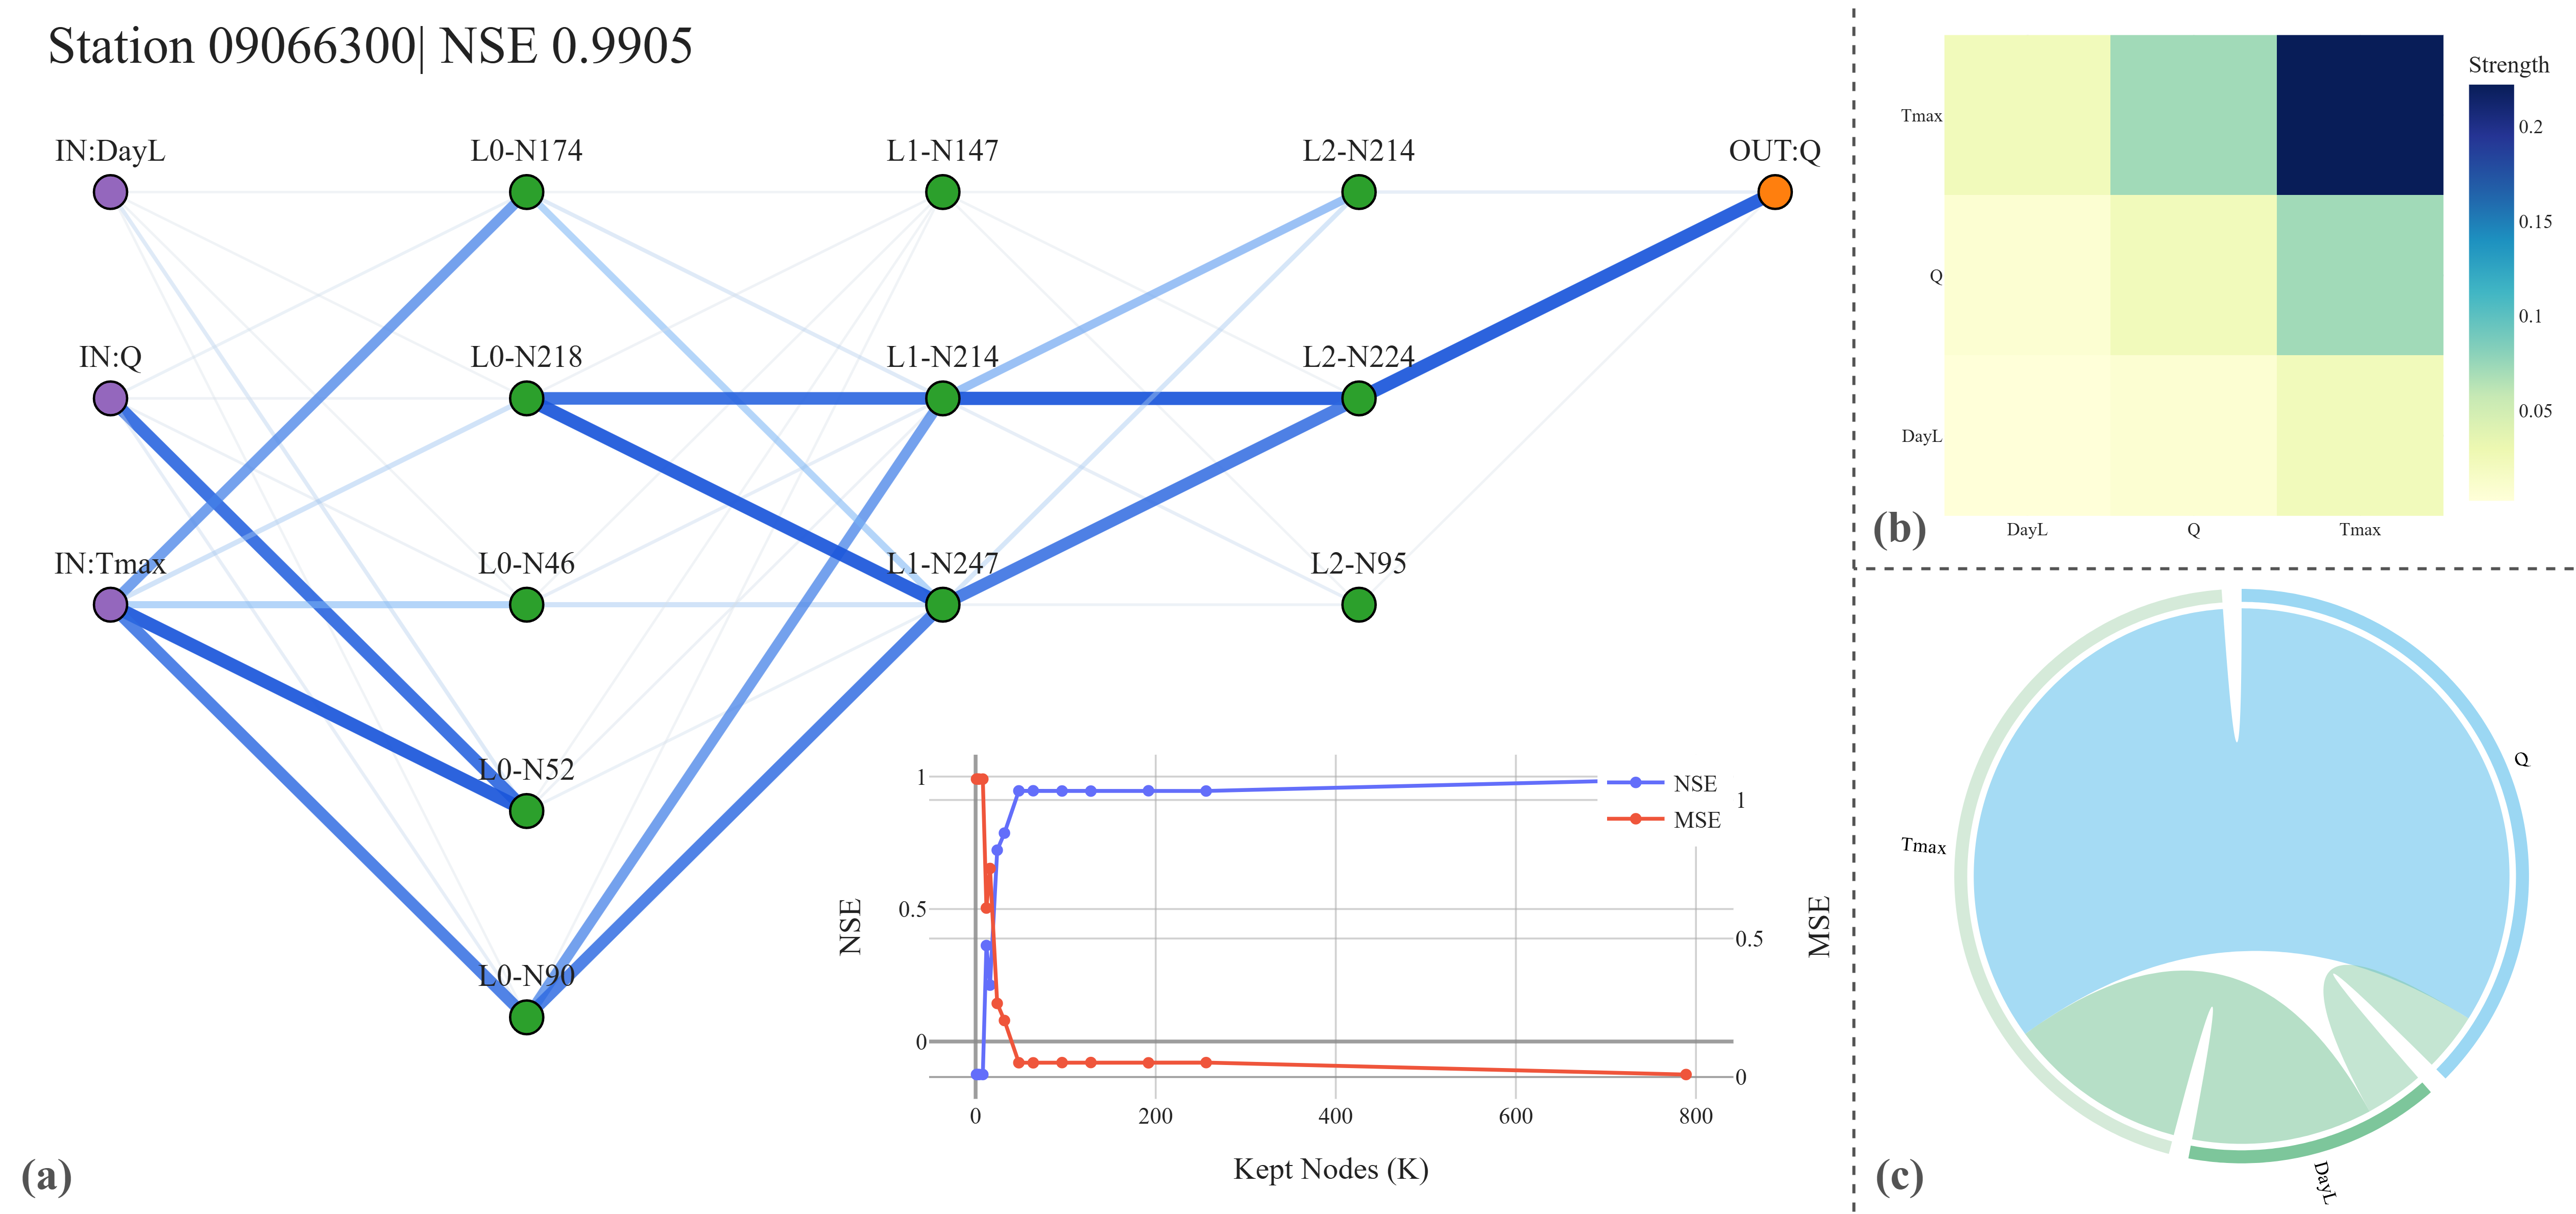
\includegraphics[width=\linewidth]{Figures/Nse_99.png}
    \caption{\textbf{Extracted sparse circuit and interpretability analysis for a representative inland station with very good performance (NSE = 0.9905).} (a) Core circuit structure and training dynamics, where lighter-colored edges indicate weaker contributions and less important pathways. (b) Interaction strength between input variables, illustrating pairwise dependencies. (c) Contribution of each input variable to streamflow prediction.}
    \label{fig:inland_circuit}
\end{figure}

For a representative station with good performance (Station ID: 01439500, \textit{Bush Kill at Shoemakers, PA}, 41.09°N, 75.04°W, NSE = 0.7366), the extracted circuit exhibits a moderately sparse structure (Fig.~\ref{fig:good_station}). Compared to the inland very good station, more input variables contribute to the prediction, including precipitation (P), streamflow (Q), and radiation-related variables. The circuit shows a more distributed information flow\cite{wang2022interpretabilitywildcircuitindirect}, indicating that multiple sub-processes are active simultaneously. Interaction analysis further suggests that Q remains dominant but is strongly coupled with precipitation, which can be interpreted as an event-response pathway where rainfall inputs are filtered by antecedent wetness and then transmitted to discharge\cite{BURN2023129075}. Overall, the extracted circuit still preserves the main predictive capability, though with increased complexity and reduced sparsity.

\begin{figure}[ht]
    \centering
    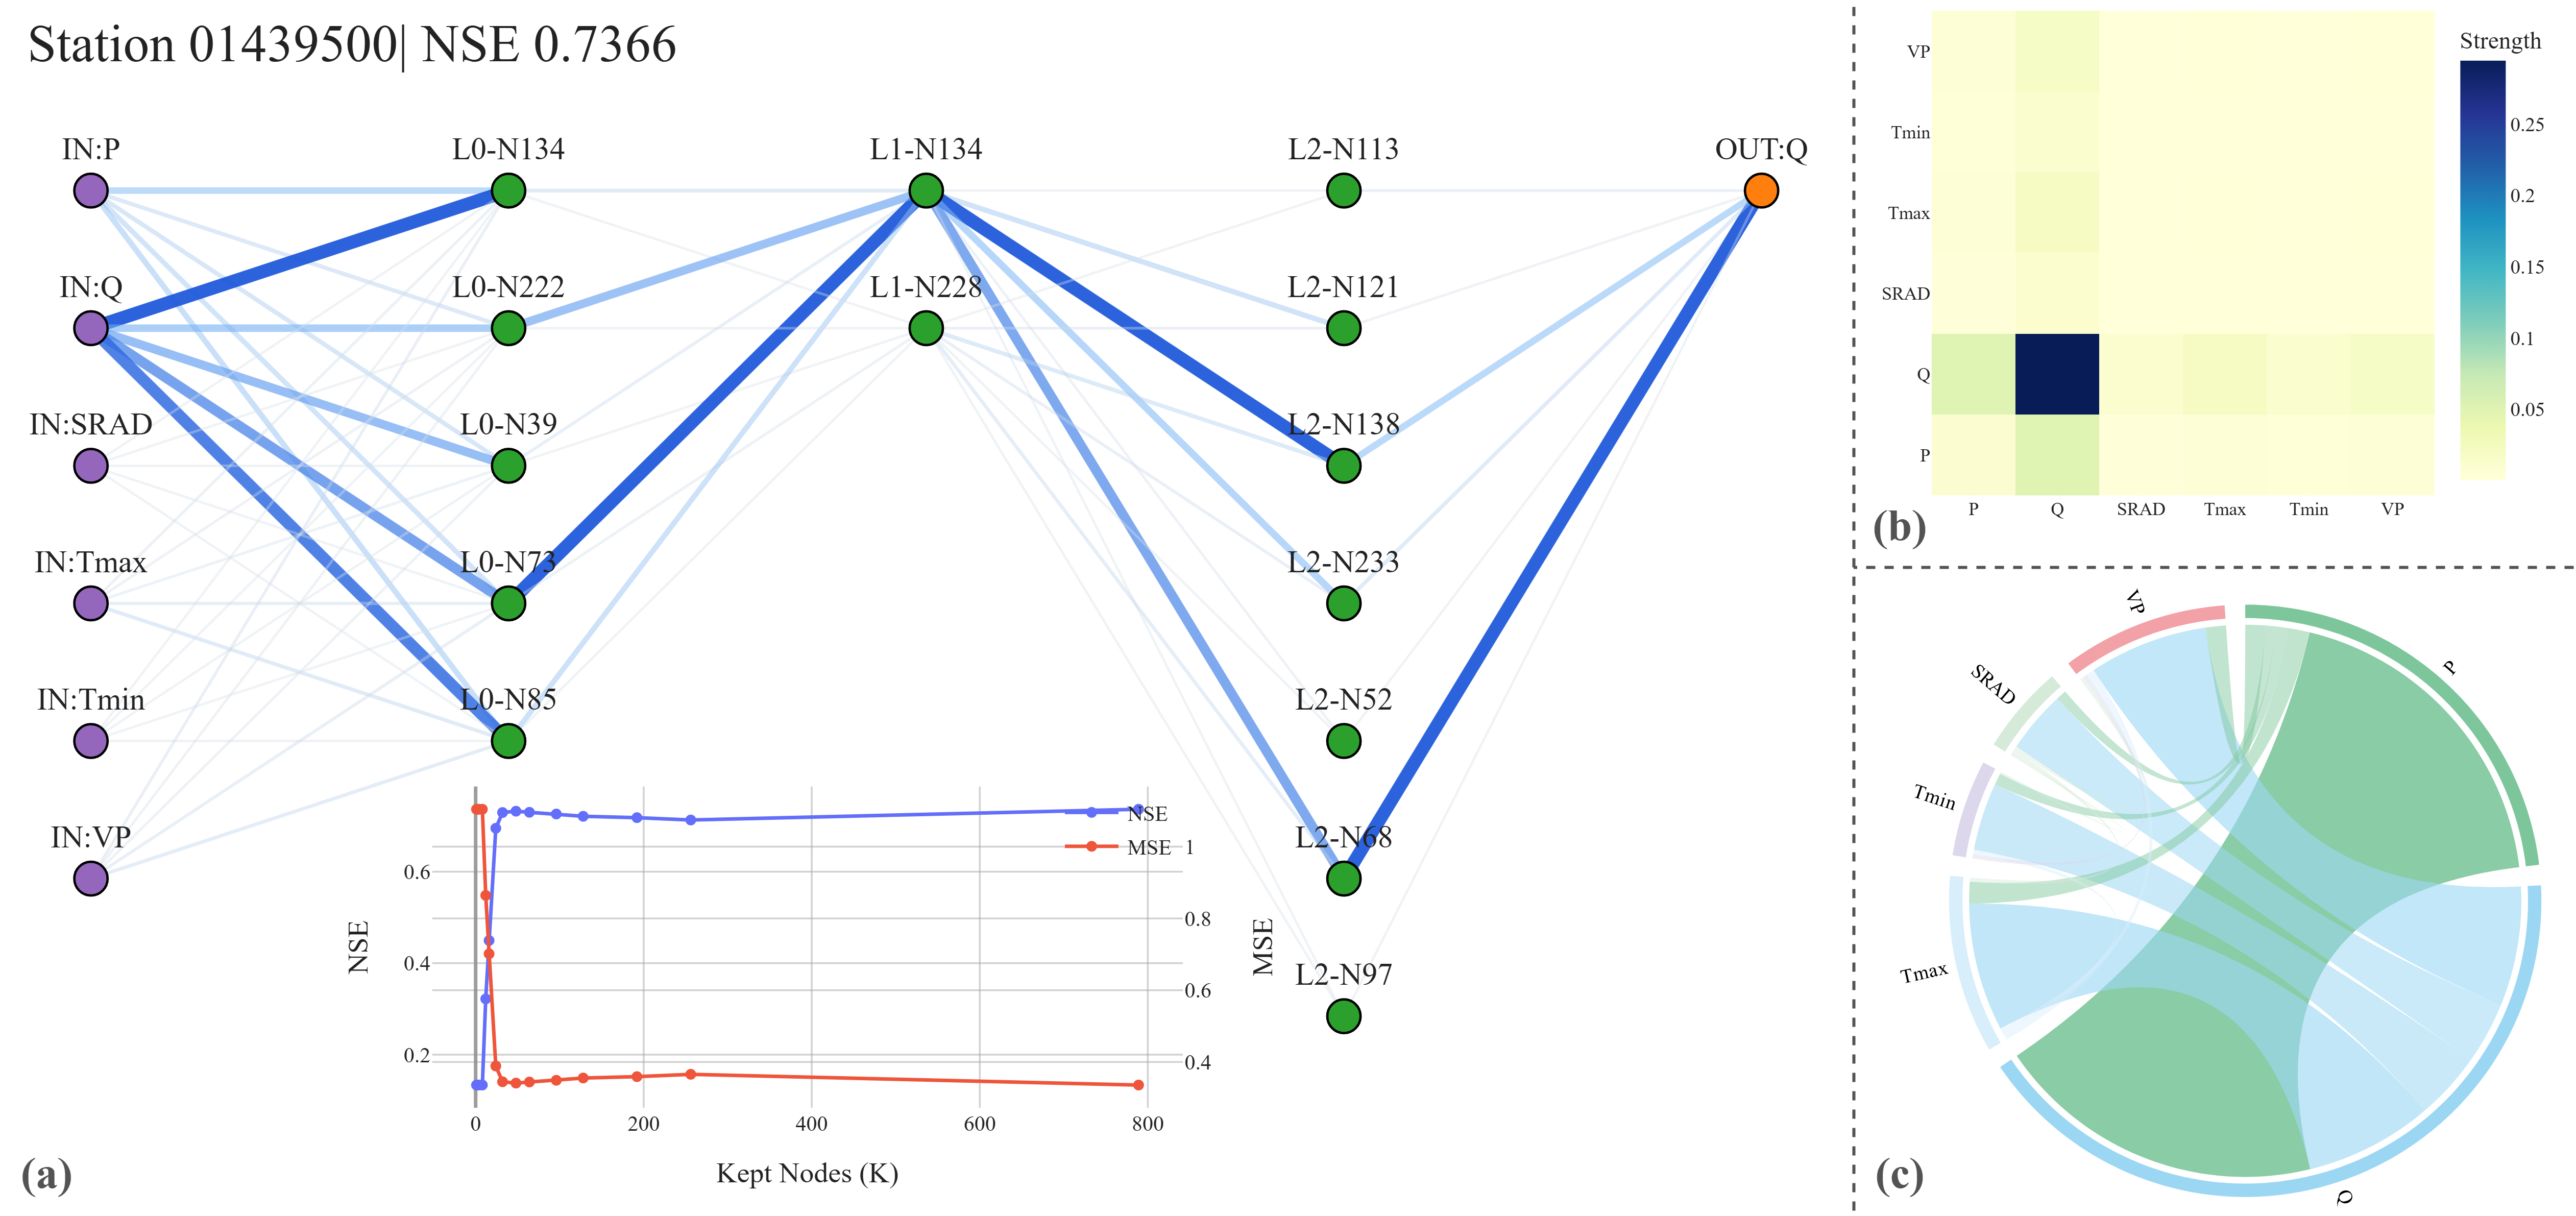
\includegraphics[width=\linewidth]{Figures/Nse_73.png}
    \caption{Extracted sparse circuit for a representative station with good performance (NSE = 0.7366).}
    \label{fig:good_station}
\end{figure}

For a representative station with satisfactory performance (Station ID: 03504000, \textit{Nantahala River near Rainbow Springs, NC}, 35.13°N, 83.62°W, NSE = 0.6217), the extracted circuit becomes less structured and more diffuse (Fig.~\ref{fig:satisfactory_station}). Although streamflow (Q) still dominates the prediction, other variables such as radiation (SRAD) and DayL show weaker and less consistent contributions. The interaction patterns are less pronounced, suggesting that no single robust hydrological pathway is cleanly separated from competing signals. In addition, the circuit retains more redundant connections, indicating that the sparsity-inducing process is less effective in isolating a compact predictive core\cite{openai_weight_sparse_transformers}. This reflects the reduced model performance and highlights the increasing difficulty of extracting clear and physically consistent hydrological knowledge in lower-performing cases\cite{ORTH2015147}.

\begin{figure}[ht]
    \centering
    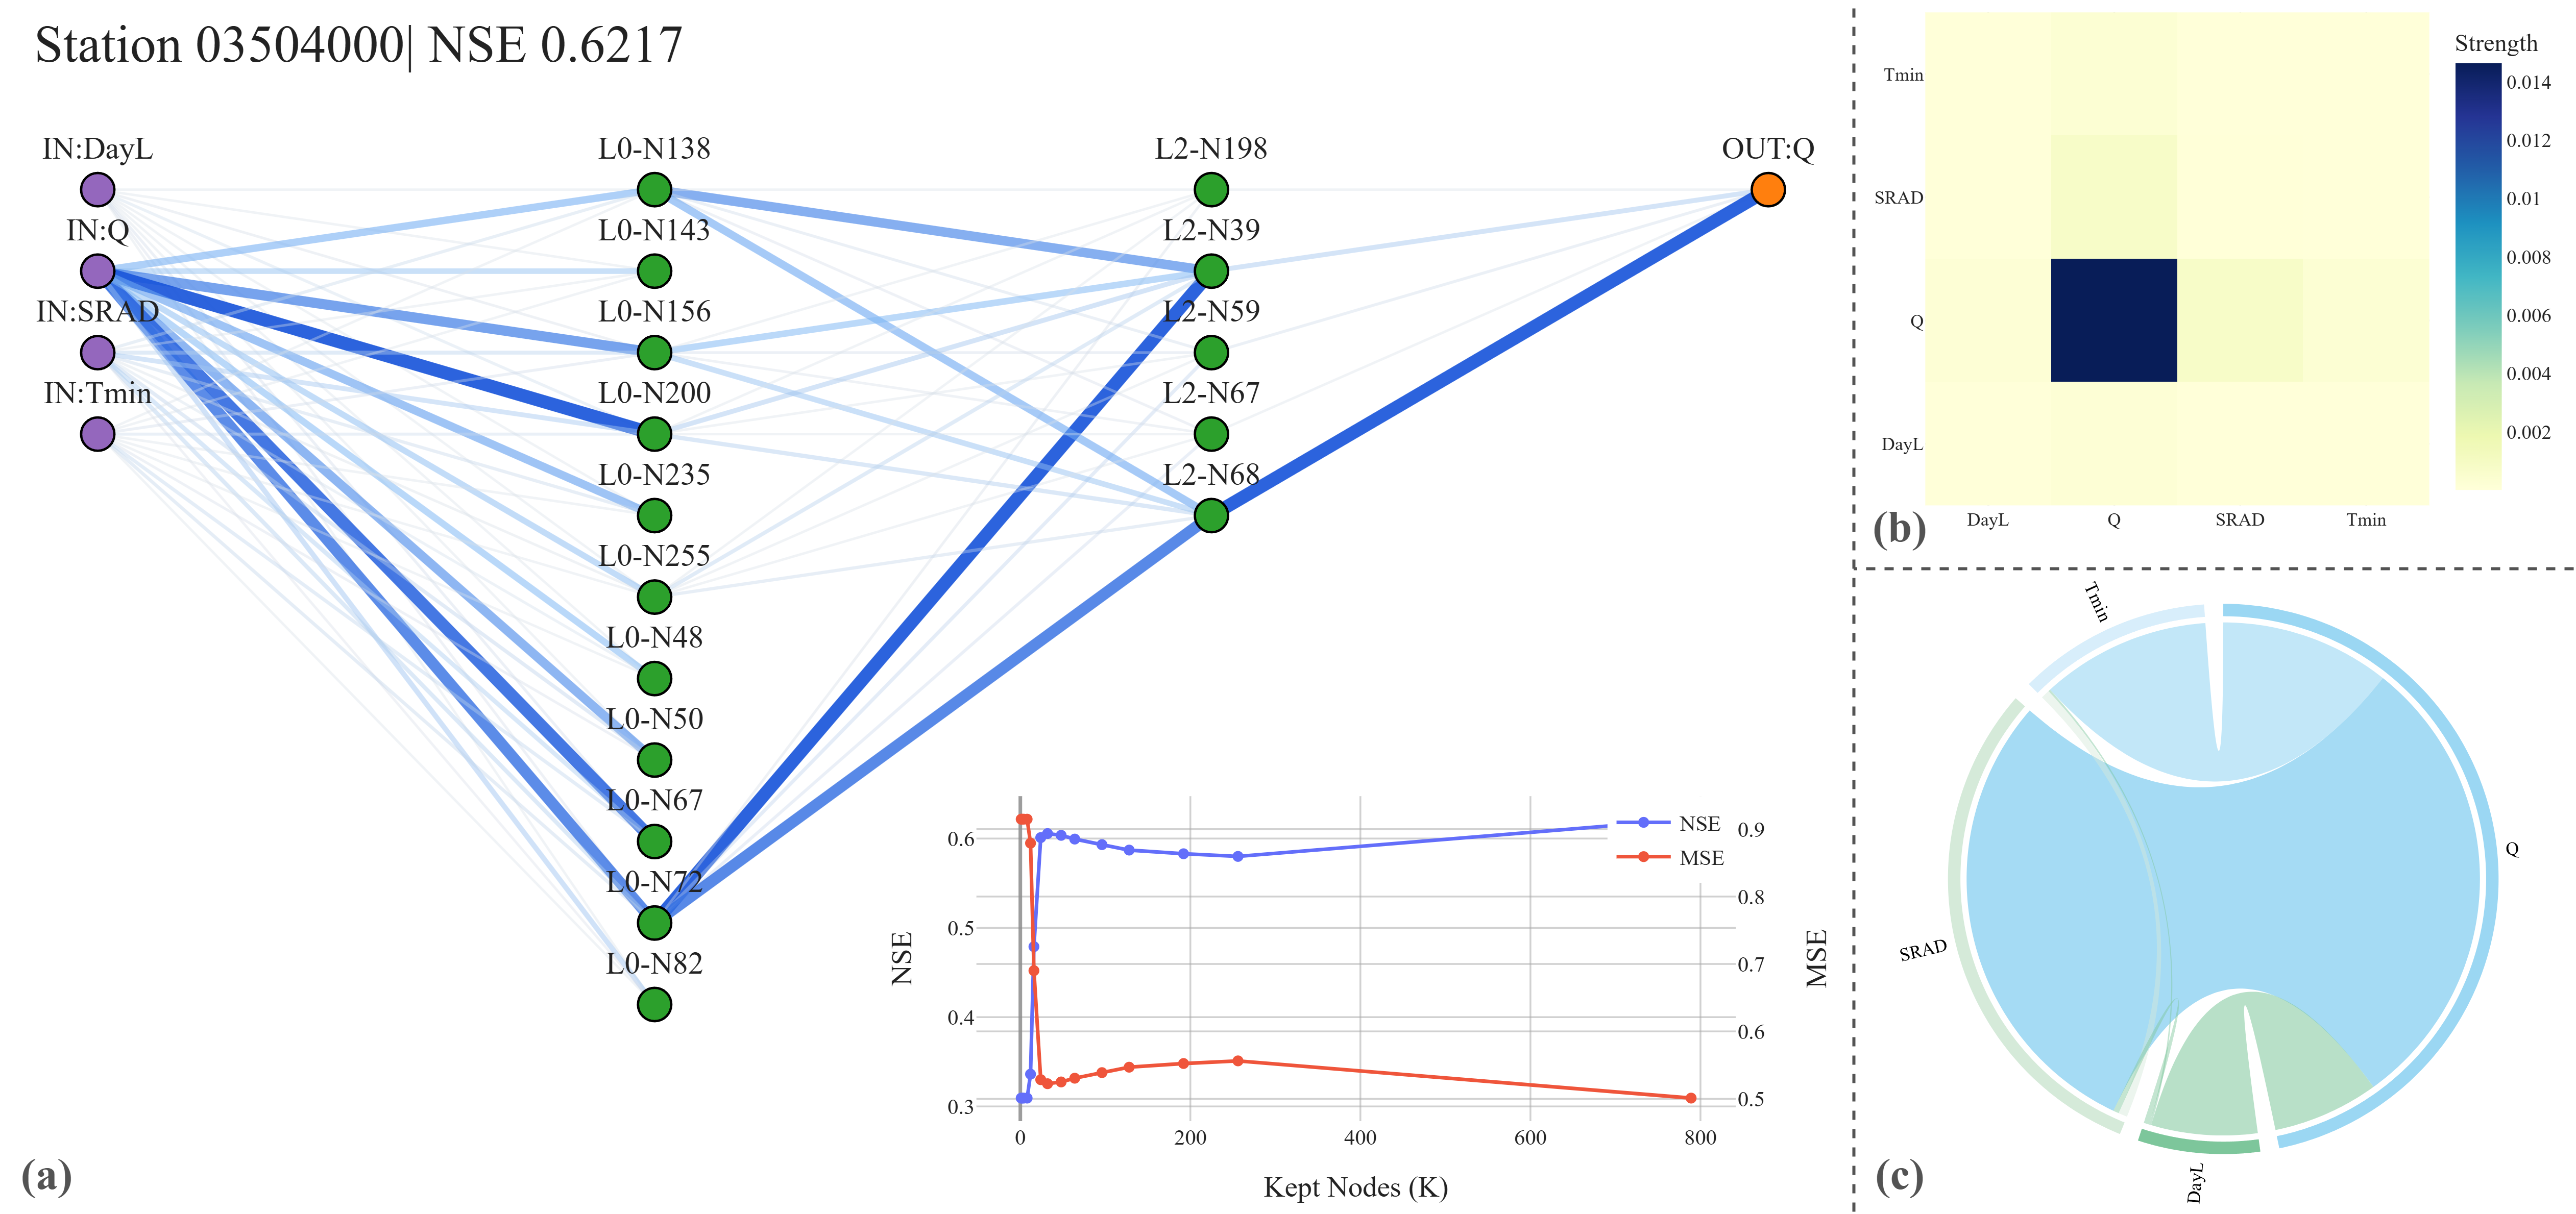
\includegraphics[width=\linewidth]{Figures/Nse_62.png}
    \caption{Extracted sparse circuit for a representative station with satisfactory performance (NSE = 0.6217).}
    \label{fig:satisfactory_station}
\end{figure}

Comparing the three representative stations, a clear pattern emerges: as predictive performance decreases, the extracted circuits become less sparse and more diffuse. High-performing stations exhibit compact and structured pathways that map to identifiable hydrological modes, while lower-performing stations show increased redundancy, weaker interaction coherence, and less stable knowledge-level interpretation.

\FloatBarrier